\documentclass[12pt]{article}

% Packages
\usepackage[margin=1in]{geometry}
\usepackage{fancyhdr}
\usepackage{amsmath, amsthm, amssymb, physics}
\usepackage{dirtree, graphicx}

% Page Style
\fancypagestyle{plain}{
    \fancyhf{}
    \renewcommand{\headrulewidth}{0pt}
    \renewcommand{\footrulewidth}{0pt}
    \fancyfoot[R]{\thepage}
}
\pagestyle{plain}

% Problem Box
\setlength{\fboxsep}{4pt}
\newsavebox{\savefullbox}
\newenvironment{fullbox}{\begin{lrbox}{\savefullbox}\begin{minipage}{\dimexpr\textwidth-2\fboxsep\relax}}{\end{minipage}\end{lrbox}\begin{center}\framebox[\textwidth]{\usebox{\savefullbox}}\end{center}}
\newenvironment{pbox}[1][]{\begin{fullbox}\ifx#1\empty\else\paragraph{#1}\fi}{\end{fullbox}}

% Options
\renewcommand{\thesubsection}{\thesection(\alph{subsection})}
\allowdisplaybreaks
\addtolength{\jot}{4pt}
\theoremstyle{definition}
%\setlength{\parindent}{0pt}


% Default Commands
\newtheorem{proposition}{Proposition}
\newtheorem{lemma}{Lemma}
\newcommand{\ds}{\displaystyle}
\newcommand{\isp}[1]{\quad\text{#1}\quad}
\newcommand{\N}{\mathbb{N}}
\newcommand{\Z}{\mathbb{Z}}
\newcommand{\Q}{\mathbb{Q}}
\newcommand{\R}{\mathbb{R}}
\newcommand{\C}{\mathbb{C}}
\newcommand{\eps}{\varepsilon}
\renewcommand{\phi}{\varphi}
\renewcommand{\emptyset}{\varnothing}
\newcommand{\pfrac}[2]{\left(\frac{#1}{#2}\right)}

% Extra Commands
\newcommand{\tsum}{\textstyle\sum\limits}

% Document Info
\fancypagestyle{title}{
    \renewcommand{\headrulewidth}{0.4pt}
    \setlength{\headheight}{15pt}
    \fancyhead[R]{Harry Coleman}
    \fancyhead[L]{GEOG 191 Lab 7}
    \fancyhead[C]{March 5, 2021}
}

% Begin Document
\begin{document}
\thispagestyle{title}


\begin{pbox}[1]
    Solve the problem as a linear program (no integer requirements). Report the solution and solver details. Discuss whether the solution makes sense for planning and management decision making.
\end{pbox}

\begin{center}
    \includegraphics[width=0.9\textwidth]{code1.png}
\end{center}

After $348$ iteration of the simplex dual algorithm, Xpress finds an LP optimal solution with an objective value of about $576436$. However, the decision variable values are almost exclusively fractional between $0.97$ and $0.99$. Seeing as their meaning is only defined for binary values, we cannot directly interpret this as a solution to the original problem.

If we assume that this result contains a meaningful solution to the original problem, then we would want to find some rule to interpret each decision variable as binary. For example, we might select the units which have positive decision values, but this would include almost every site, violating our adjacency constraints. Alternately, we might select the sites using some minimum threshold, but any choice of threshold would be fairly arbitrary and, again, it would be unlikely that this would satisfy the adjacency constraints. 

It may be possible to find some such rule which produces a valid solution, but from what we know about the implementation, we can say with reasonable certainty that this would be no better than randomly guessing a solution. To see why this is the case, consider how the adjacency constraint is implemented:
\[
    Mx_i + \tsum_{j \in \Omega_i} x_j \leq M, \quad \forall i,
\]
where $\Omega_i$ is the set of units adjacent to unit $i$ and $M$ is an arbitrarily large constant, no less than the total number of units. Assuming that each decision variable is binary, we will verify that this inequality actually implements the desired adjacency constraint. For a fixed index $i$, if $x_i = 1$, then the above constraint becomes
\[
    M + \tsum_{j \in \Omega_i} x_j \leq M
        \implies \tsum_{j \in \Omega_i} x_j \leq 0.
\]
And since $x_j \geq 0$ for each $j \in \Omega_i$, then we must have $x_j = 0$ for all $j \in \Omega_i$. That is, if unit $i$ is selected, then none of the adjacent units are selected. Conversely, suppose $x_j = 1$ for some $j \in \Omega_i$. Then it is also the case that $i \in \Omega_j$, and repeating the same argument, we must have $x_i = 0$. Hence, $x_i = 1$ if and only if $x_j = 0$ for all $j \in \Omega_i$. In other words, no pair of adjacency units are simultaneously selected, which is precisely the desired adjacency constraint.

However, this argument falls apart if we do not require the decision variables to be binary. In particular, it is supported by the fact that if a given decision variable is strictly less than one, then it must be zero. But allowing fractional values enables the decision variable to simply take on a value very slightly less than $1$. Explicitly, each decision variable need not decrease by more than $1/M$ to accommodate each additional neighbor. Since this is such a small penalty, the solver essentially ignores the constraint, producing values around $0.98$. We can be reasonably sure that this result contains no useful information about the actual problem.



\newpage
\begin{pbox}[2]
    Using the linear program, construct a branch and bound tree to resolve any observed fractional decision variables (stop after 10 branches).
\end{pbox}

\vspace{4pt}
\dirtree{%
.1 0: LP $576435$, branch at $x_1 = 0.99$.
    .2 1 $x_1 \leq 0$: LP $574139$, branch at $x_2 = 0.99$.
        .3 3 $x_2 \leq 0$: LP $571830$, branch at $x_3 = 0.98$.
            .4 7 $x_3 \leq 0$: LP $569557$.
            .4 8 $x_3 \geq 1$: LP $563966$.
        .3 4 $x_2 \geq 1$: LP $571870$, branch at $x_3 = 0.98$.
            .4 9 $x_3 \leq 0$: LP $569597$.
            .4 10 $x_3 \geq 1$: LP $564006$.
    .2 2 $x_1 \geq 1$: LP $571902$, branch at $x_2 = 0.99$.
        .3 5 $x_2 \leq 0$: LP $569593$, branch at $x_3 = 0.98$.
            .4 11 $x_3 \leq 0$: LP $567320$.
            .4 12 $x_3 \geq 1$: LP $561705$.
        .3 6 $x_2 \geq 1$: LP $569633$, branch at $x_3 = 0.98$.
            .4 13 $x_3 \leq 0$: LP $567360$.
            .4 14 $x_3 \geq 1$: LP $561745$.
}
\vspace{4pt}

To construct the branch and bound tree, we use the same code as above with added constraints at each node. When solving the problem at at node, we include all the constraints of its parent and one new constraint for the variable which is being branched at. For example, the following code is included when solving at node 9:
\begin{center}
    \includegraphics[width=0.2\textwidth]{code1b.png}
\end{center}
The appropriate lines are commented/uncommented for each node.





\newpage
\begin{pbox}[3]
    Solve the problem using Xpress as an integer program. Report the solution and solver details. Discuss whether the solution makes sense for planning and management decision making.
\end{pbox}

\begin{center}
    \includegraphics[width=0.9\textwidth]{code2.png}
\end{center}

With the added integer constraints, the solver finds an optimal binary solution with an objective value of $231892$. This time, each decision variable is binary, so we are able to interpret it as a solution to the original problem. In particular, the units whose corresponding decision variable has a value of $1$ should be selected. The selected units are as follows:
\begin{verbatim}
1, 2, 4, 8, 9, 15, 21, 23, 26, 29, 30, 31, 33, 37, 38, 41, 42, 44, 48, 49,
56, 58, 62, 63, 64,65, 66, 67, 73, 78, 80, 82, 83, 86, 88, 91, 93, 99, 100,
107, 114, 116, 119, 120, 122, 124, 127, 129, 131,132, 138, 139, 141, 145,
149, 154, 155, 156, 158, 163, 165, 166, 167, 173, 175, 178, 179, 185, 186,
187, 189, 190, 194, 198, 202, 207, 209, 214, 215, 217, 220, 223, 225, 228,
231, 234, 235, 239, 246, 247, 248, 251, 253, 256, 263, 266, 268, 273, 274,
275, 277, 283, 284, 285, 295, 300, 306, 308, 312, 314, 317, 318, 322, 330,
332, 333, 336, 338, 339, 342, 344, 346, 347, 349, 351.
\end{verbatim}


\begin{pbox}[4]
    Map the solution using the corresponding ArcGIS data layer.
\end{pbox}

The selected units are marked in blue.

\begin{center}
    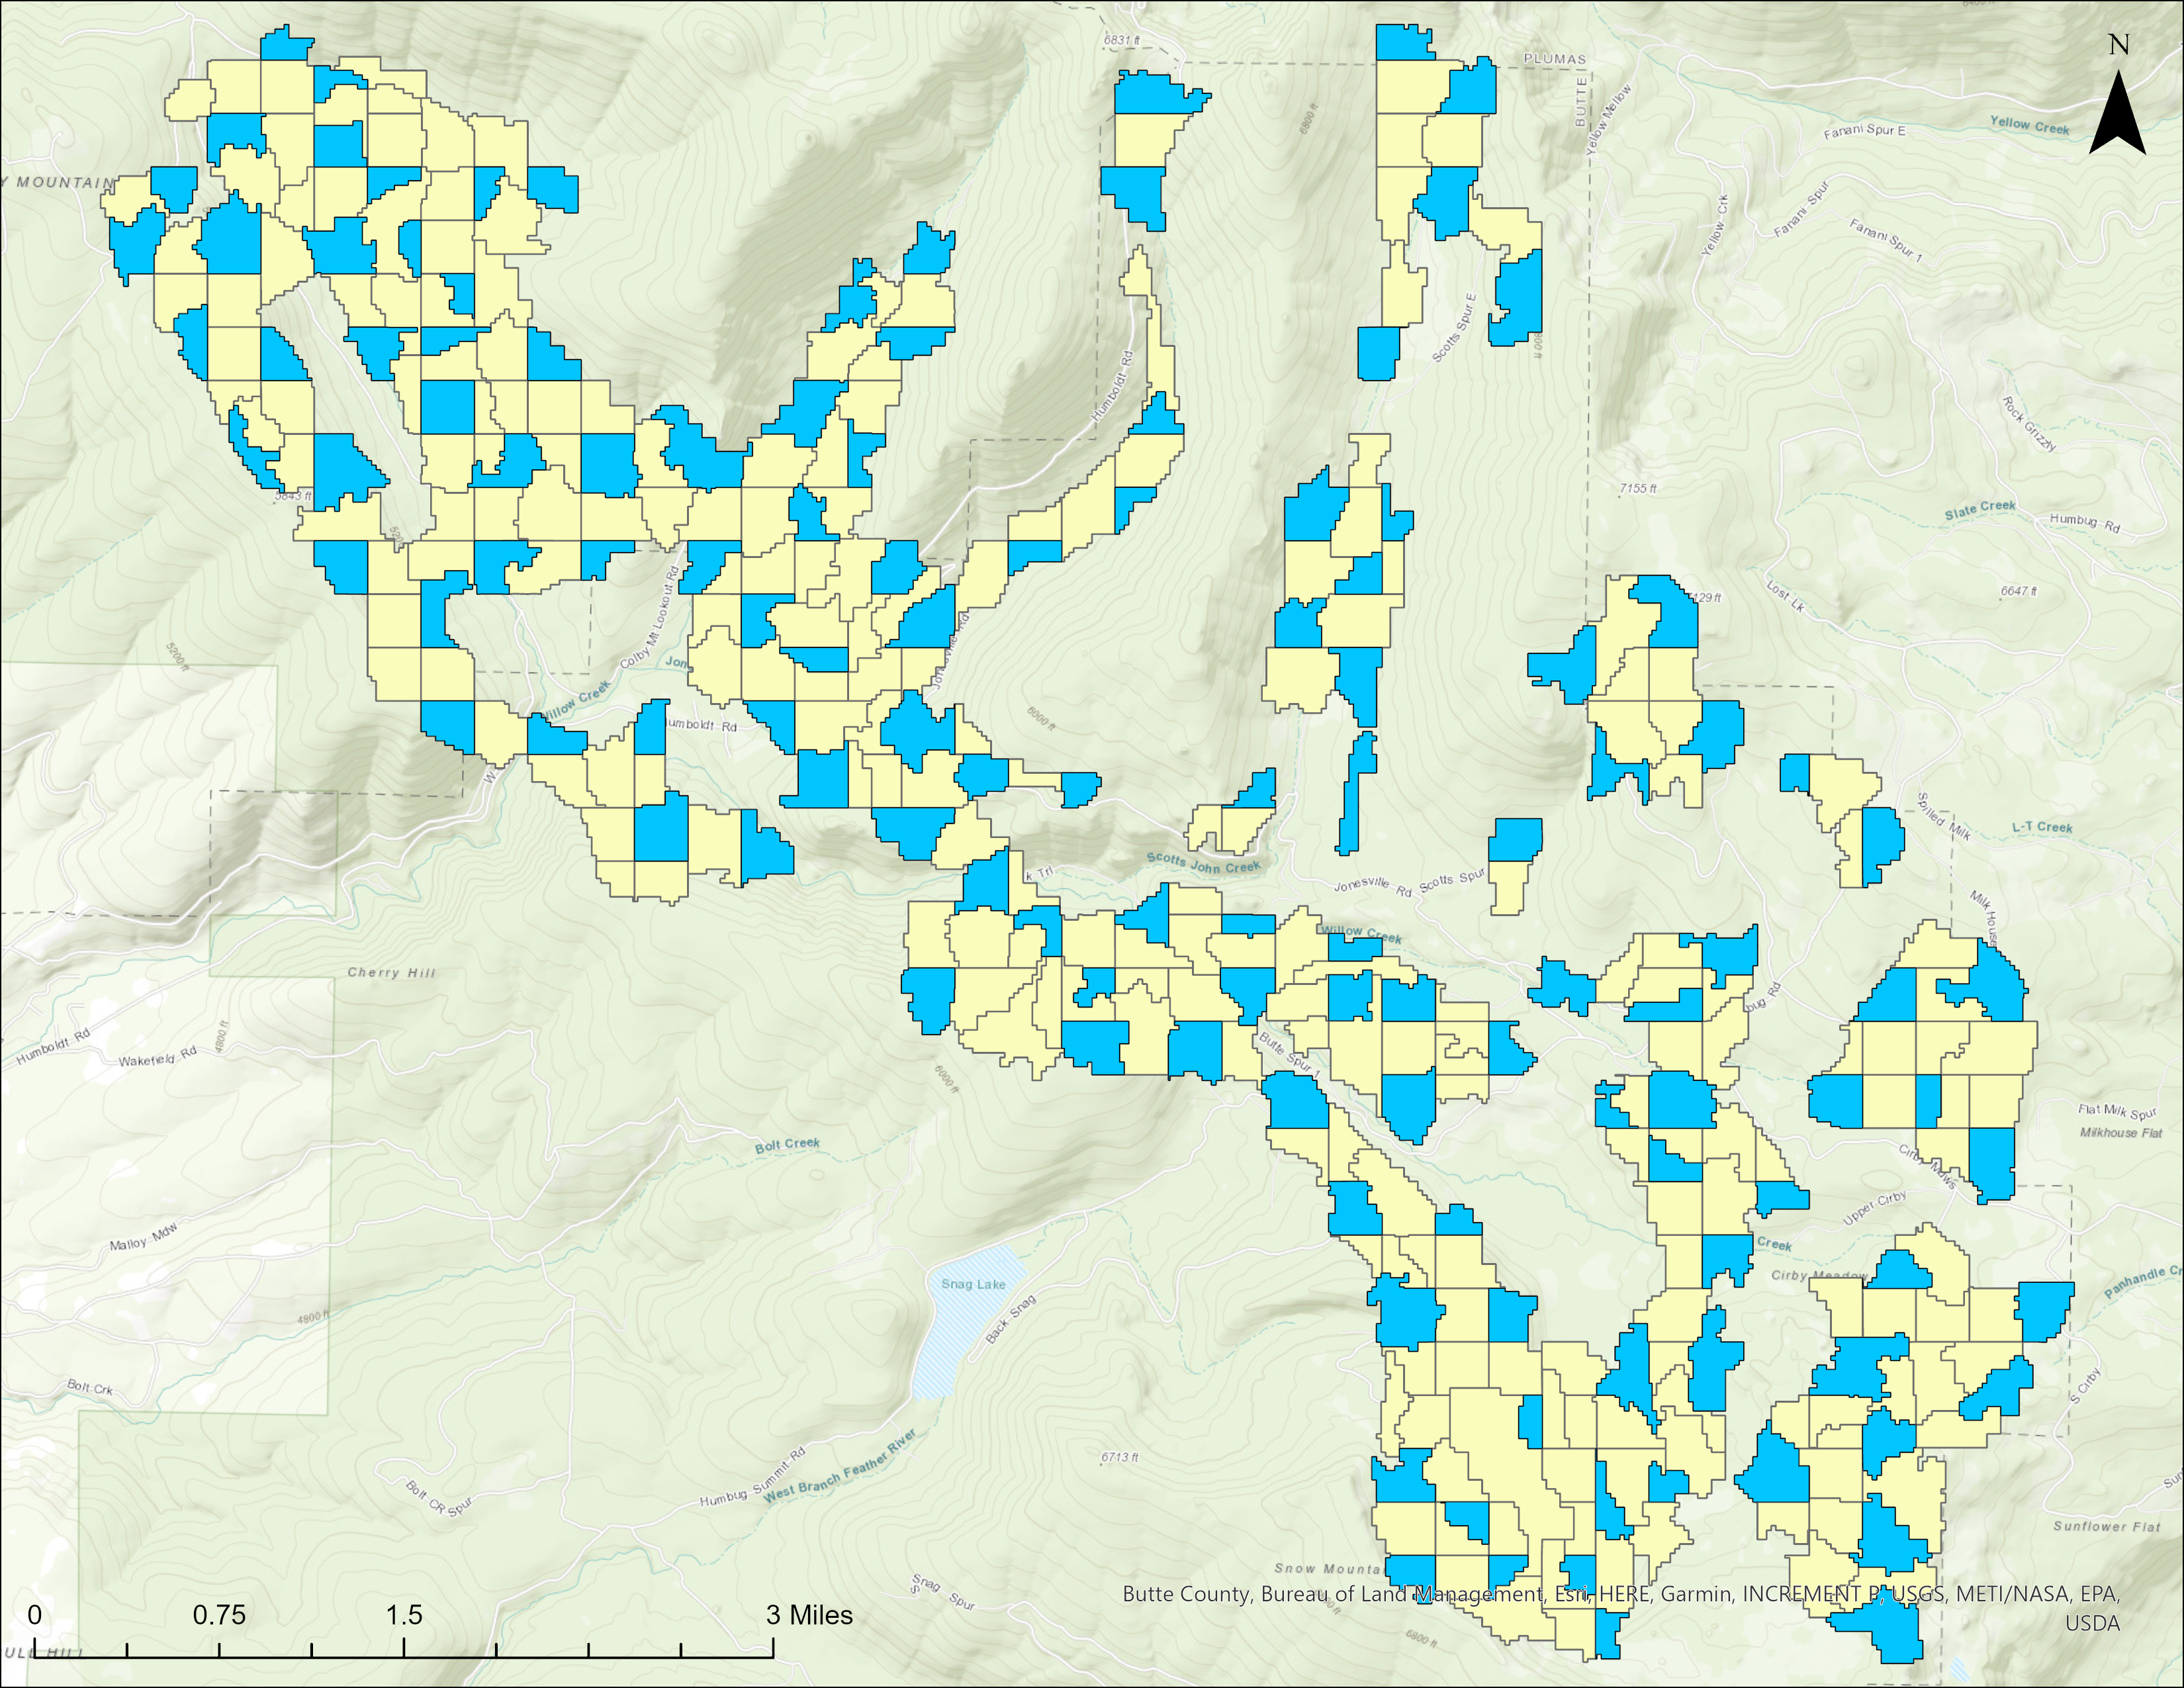
\includegraphics[width=\textwidth]{map.png}
\end{center}


\end{document}